\documentclass[a4]{report}
\def\atitle{Rheometor Control System: Hardware Overview}
\def\theauthor{Christopher Boyle}
\def\thewords{4466}

\def\br{\newline \newline \noindent}


% Imports
\usepackage{graphicx}
\usepackage[a4paper]{geometry}
\usepackage{fancyhdr}
\usepackage[english]{babel}
\usepackage{etoolbox}
\usepackage{url}
\usepackage[hidelinks]{hyperref}
\usepackage{subcaption}

% Unused packages
%\usepackage{placeins}
%\usepackage{fancyref}
%\usepackage[comma,authoryear]{natbib}
%\usepackage{lipsum}

% Settings
\geometry{top=2cm, bottom=2.5cm, left=3cm, right=2.5cm}
\patchcmd{\chapter}{\thispagestyle{plain}}{\thispagestyle{plain}}{}{}
\patchcmd{\section}{\thispagestyle{plain}}{\thispagestyle{plain}}{}{}
\patchcmd{\subsection}{\thispagestyle{plain}}{\thispagestyle{plain}}{}{}
\setcounter{secnumdepth}{0}
\renewcommand{\theequation}{\arabic{equation}}
\renewcommand\UrlFont{\rmfamily\itshape}
\setlength{\fboxsep}{0pt}
\setlength{\fboxrule}{0pt}
\def\achapter{preamble}
%%%% TEMPLATES
\iffalse


%%%EQUATION

	\begin{equation}
		(THE EQUATION)
		\label{EQUATION REF}
	\end{equation}


%%%FIGURE

	\begin{figure}[!htb]
		\centering
		\fbox{\includegraphics[scale=SCALE]{IMAGE LOCATION}}
		\caption{CAPTION}
		\label{FIGURE REF}
	\end{figure} \newline  \noindent

%%%BULLET POINT LIST
	\begin{itemize}
	\item
	\end{itemize}

\fi
%%%%

% Header/footer preamble
\fancyhf{}
\fancypagestyle{plain}{
	\renewcommand{\headrulewidth}{0.4pt}
	\renewcommand{\footrulewidth}{0.4pt}
%	\fancyhead[L]{\atitle}
	\fancyhead[L]{\achapter}
	\fancyhead[R]{\theauthor}
	\fancyfoot[L]{\today}
	\fancyfoot[R]{\thepage}
}
\pagestyle{plain}

\begin{document}
%%%%%%%%%%%%%%%%%%%%%%%%%% TITLE PAGE
	\begin{titlepage}
		\makebox[\textwidth][c]{
\includegraphics[scale=1]{images/titleheader.png}}
		\centering
		\vskip4cm
		{
			\bfseries\Large
			Department of Chemical \& Process Engineering\\
			\vskip1cm
			MEng in Chemical \& Process Engineering\\
			18530
			\vskip3cm
			\LARGE\atitle
		}
		\vskip3cm
		\begin{flushleft}
			\vskip3cm
			Your name: \theauthor \hfill Date: \today
			\vskip1cm
			Organisation: University of Strathclyde, Department of Chemical \& Process Engineering\newline% \newline
			In-house Supervisor: Dr. Leo Lue \newline% \newline
			Academic Supervisor:  Dr. Leo Lue
		\end{flushleft}
	\end{titlepage}
	
	% Contents Page
	\def\achapter{Contents}
	\tableofcontents
	
	\pagenumbering{arabic}
	\setcounter{page}{1}
	
%=====------++++++=====------++++++=====------++++++=====------++++++=====------++++++=====------++++++=====------++++++=====------++++++=====------++++++=====------++++++=====------++++++=====------++++++=====------++++++=====------++++++=====------++++++=====------++++++
                                                               
	\chapter{Introduction}
	
	This document details the hardware used in the Raspberry Pi Rheometer system.
	
	\chapter{Background}
	
	\section{Components}
	
	\subsection{Resistor}
	
	When electricity flows down a wire (any wire) it loses energy. This can be seen by measuring the current loss (or the heat gain). This is due to the resistance of the wire. Most wire is designed to have as low a resistance as possible so that the power loss is as small as possible, and so that the physical circuit works like the theoreticla circuit. Some wire is designed to have a resistance - so called resistance wire. This is used in heating elements in kettles, electric hobs, electronic cigarettes, etc. There are small components which contain high resistance wire these are called resistors. Used primarily to reduce voltage and/or current in a circuit.
	
	\subsection{Potentiometer}
	
	A potentiometer is a kind of variable resistor. It consists of a fixed resistor with a wiper that sweeps accross the resistor. This means that the resistance between the wiper terminal and the other terminals can be varied (see Figure \ref{figpot}).
	
	\begin{figure}[!htb]
		\centering
		\fbox{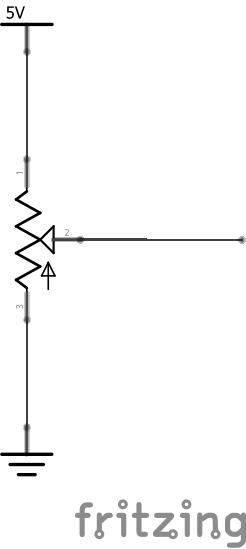
\includegraphics[scale=1]{otherimgs/pot.png}}
		\caption{Potentiometer}
		\label{figpot}
	\end{figure}
	
	\section{Useful Concepts/Equations}
	
	\subsection{Ohm's Law}
	
	Ohm's law is the relationship between resistance, current, and voltage in an electronic circuit (or part of a circuit):
	
	\begin{equation}
		V= I \times R
		\label{eqnohmlaw}
	\end{equation}
	
	This fundamental equation is incredibly useful to calculate the required resistance of a resistor.
	
	\subsection{Kirchhoff's Laws}
	
	Kirchhoff's two laws describe how current and voltage behave in an electronic circuit:
	\begin{itemize}
	\item The current in a circuit is similar to the flow rate of fluid in a pipe system. The sum of the currents flowing into a point is equal to the sum of the currents flowing out. This is Kirchhoff's First Law. 
	\item Voltage can be thought of like fluid pressure in system of pipes; the fluid loses pressure over obstacles in the same way the circuit loses voltage over a resistor/lamp/motor/whatever component. The sum of the voltages around a loop of a circuit is always zero. This means that the voltages in wires coming from a branch are equal (i.e. when a wire splits into two, the voltages are equal on all three wires).
	\end{itemize}
	\begin{figure}[!htb]
		\centering
		\fbox{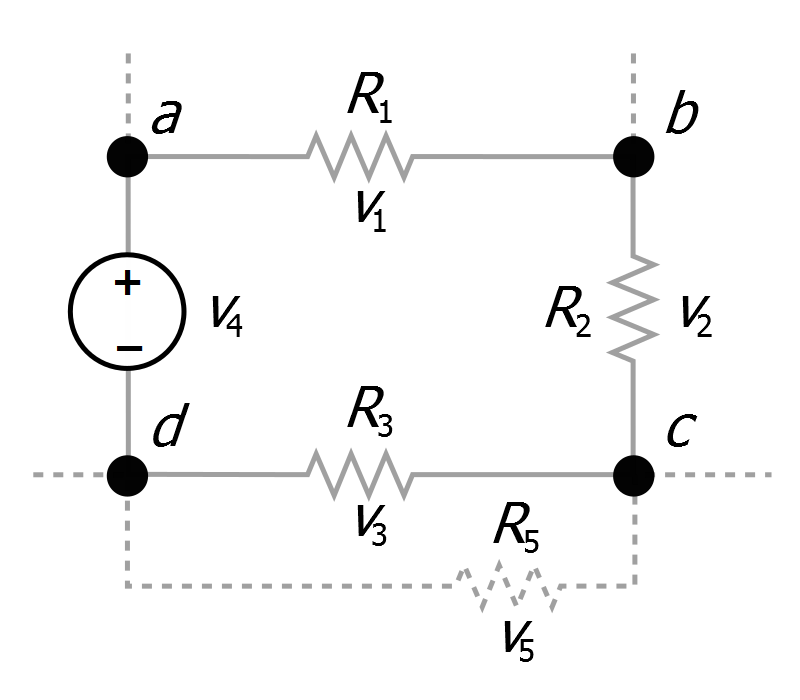
\includegraphics[scale=0.2]{otherimgs/k2law.png}}
		\caption{Kirchhoff's 2nd Law: V1 + V2 + V3 - V4 = 0}
		\label{figk2law}
	\end{figure}
	
	\subsection{Voltage Dividers}
	
	A voltage divider is a very useful and very simple circuit used to reduce a voltage to a defined level. A voltage divider is simply two resistors connected to a power source (see Figure \ref{figvdiv}). The voltage is split between each resistor, proportional to their resistances. There is a wire tapped into the point between the resistors, the voltage on this wire is equal to the voltage accross the second resistor. This voltage can be calculated using Equation \ref{eqnvdiv}. The figure shows a voltage divider with a 5v power source. Assuming the two resistors are the same, then the middle wire has a voltage of 2.5v.
	
	\begin{equation}
		V_{wire} = V_{supply} * \frac{R_2}{R_1+ R_2}
		\label{eqnvdiv}
	\end{equation}
	
	\begin{figure}[!htb]
		\centering
		\fbox{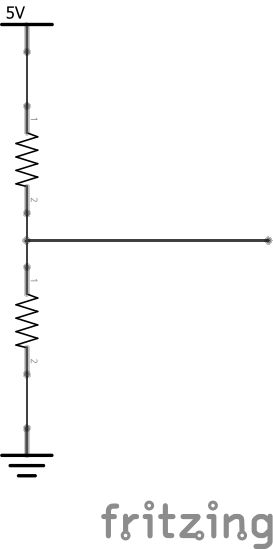
\includegraphics[scale=1]{otherimgs/vdiv.png}}
		\caption{Simple Voltage Divider}
		\label{figvdiv}
	\end{figure}

\end{document}